\documentclass[xcolor={dvipsnames}]{beamer}
\mode<presentation>
{
  \usetheme{default}      % or try Darmstadt, Madrid, Warsaw, ...
  \usecolortheme{default}
  \usepackage{beamerthemesplit}% or try albatross, beaver, crane, ...
  \usefonttheme{default}  % or try serif, structurebold, ...
  \setbeamertemplate{navigation symbols}{}
  \setbeamertemplate{caption}[numbered]
}
\usepackage[english]{babel}
\usepackage[utf8x]{inputenc}
\usepackage{tikz}
\usepackage{pgfplots}
\usepackage{pgf-pie}
\title[Analizador Lexico\hspace{0.5cm}\insertframenumber/\inserttotalframenumber]{Proyecto 1: Analizador Lexico }
\author{ Esteban Durán \and David Hernández  \and Diego Mendez   }
\institute{Instuto Tecnológico De Costa Rica\\ Compiladores e Intérpretes}
\date{27-04-2022}
\begin{document}
\begin{frame}
  \titlepage
\end{frame}

\begin{frame}{Scanning and Flex}
El proceso de scanning es una fase de la compilación la cual se encarga de tomar el código fuente de entrada (el cual ya pasó por la etapa de preprocesado) y generar tokens que sean representativos del código escrito en este. Cada uno de estos tokens está compuesto por uno o más símbolos que lo representan, este conjunto se le conoce como "Lexema".
\begin{figure}
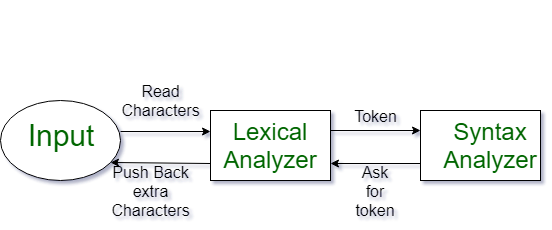
\includegraphics[width=9cm]{phases.png}
\end{figure}
  \end{frame}

%\section{Problem Statement}

\begin{frame}{Scanning y Flex}


  Flex genera este scanner de manera sencilla. Este procesa cada token de un archivo de entrada donde uno a uno se extraen mediante una función propia de Flex. Este conjunto de tokens por lo general siguen una string específica o un caracter que los idéntifique. Si un token lo requiere, se pueden identificar reglas mediante expresiones regulares que ayuden a extraerlo específicamente. Esto también permite crear funciones dentro del mismo scanner que permita manipular esta información según la funcionalidad del scanner.
  \begin{figure}

\includegraphics[width=3cm]{flex.jpg}
\end{figure}

\end{frame}
\begin{frame}[allowframebreaks]{Programa Fuente}
		\newline 
\newline 
\newline 
\newline 
\newline 
\newline 
\fontfamily{cmr}\selectfont\textcolor{Blue}{\colorbox{Cyan}{int}}\fontfamily{cmss}\selectfont\textcolor{Yellow}{\colorbox{Violet}{a}}\fontfamily{lmtt}\selectfont\textcolor{ForestGreen}{\colorbox{LimeGreen}{=}}\fontfamily{qag}\selectfont\textcolor{orange}{\colorbox{Yellow}{1}}\fontfamily{put}\selectfont\textcolor{white}{\colorbox{teal}{;}}\newline 
\fontfamily{cmr}\selectfont\textcolor{Blue}{\colorbox{Cyan}{char}}\fontfamily{cmss}\selectfont\textcolor{Yellow}{\colorbox{Violet}{b}}\fontfamily{lmtt}\selectfont\textcolor{ForestGreen}{\colorbox{LimeGreen}{=}}\fontfamily{put}\selectfont\textcolor{white}{\colorbox{teal}{'}}\fontfamily{cmss}\selectfont\textcolor{Yellow}{\colorbox{Violet}{ab}}\fontfamily{put}\selectfont\textcolor{white}{\colorbox{teal}{'}}\fontfamily{put}\selectfont\textcolor{white}{\colorbox{teal}{;}}\newline 
\fontfamily{cmr}\selectfont\textcolor{Blue}{\colorbox{Cyan}{int}}\fontfamily{put}\selectfont\textcolor{white}{\colorbox{teal}{(}}\fontfamily{qag}\selectfont\textcolor{orange}{\colorbox{Yellow}{20}}\fontfamily{lmtt}\selectfont\textcolor{ForestGreen}{\colorbox{LimeGreen}{+}}\fontfamily{qag}\selectfont\textcolor{orange}{\colorbox{Yellow}{0}}\fontfamily{put}\selectfont\textcolor{white}{\colorbox{teal}{)}}\fontfamily{qag}\selectfont\textcolor{orange}{\colorbox{Yellow}{33}}\fontfamily{qag}\selectfont\textcolor{orange}{\colorbox{Yellow}{0}}\fontfamily{lmtt}\selectfont\textcolor{ForestGreen}{\colorbox{LimeGreen}{=}}\fontfamily{cmss}\selectfont\textcolor{Yellow}{\colorbox{Violet}{bac}}\fontfamily{lmtt}\selectfont\textcolor{ForestGreen}{\colorbox{LimeGreen}{+}}\fontfamily{qag}\selectfont\textcolor{orange}{\colorbox{Yellow}{0}}\fontfamily{lmtt}\selectfont\textcolor{ForestGreen}{\colorbox{LimeGreen}{+}}\fontfamily{qag}\selectfont\textcolor{orange}{\colorbox{Yellow}{0}}\fontfamily{lmtt}\selectfont\textcolor{ForestGreen}{\colorbox{LimeGreen}{-}}\fontfamily{put}\selectfont\textcolor{white}{\colorbox{teal}{(}}\fontfamily{qag}\selectfont\textcolor{orange}{\colorbox{Yellow}{20}}\fontfamily{lmtt}\selectfont\textcolor{ForestGreen}{\colorbox{LimeGreen}{+}}\fontfamily{qag}\selectfont\textcolor{orange}{\colorbox{Yellow}{0}}\fontfamily{put}\selectfont\textcolor{white}{\colorbox{teal}{)}}\fontfamily{qag}\selectfont\textcolor{orange}{\colorbox{Yellow}{33}}\fontfamily{qag}\selectfont\textcolor{orange}{\colorbox{Yellow}{0}}\fontfamily{put}\selectfont\textcolor{white}{\colorbox{teal}{;}}
	\end{frame}
\begin{frame}[allowframebreaks]{Estadísticas}
		\begin{tikzpicture}
		\begin{axis}[ybar interval, xtick=empty,legend pos=outer north east,ymax=16,ymin=0]
		\addplot[style = {fill=Cyan}] coordinates { (1, 3)  (1.5, 4)};
	\addplot[style = {fill=LimeGreen}] coordinates { (1, 8)  (1.5, 4)};
	\addplot[style = {fill=gray}] coordinates { (1, 0)  (1.5, 4)};
	\addplot[style = {fill=Yellow}] coordinates { (1, 11)  (1.5, 4)};
	\addplot[style = {fill=teal}] coordinates { (1, 9)  (1.5, 4)};
	\addplot[style = {fill=Violet}] coordinates { (1, 4)  (1.5, 4)};
	\addplot[style = {fill=red}] coordinates { (1, 0)  (1.5, 4)};
	\legend{Keywords, Operator, String, Constant, Special character, Identifiers, Errors}  \end{axis}\end{tikzpicture}
	\end{frame}

	\begin{frame}[allowframebreaks]{Estadísticas}
		\begin{tikzpicture}
		\def\printonlypositive#1{\ifnum#1>0
#1
\fi}
\pie [rotate = 90,
text = legend,
before number=\printonlypositive,   
sum=auto,
every only number node/.style={text=white},
color={Cyan,LimeGreen,gray,Yellow,teal,Violet,red}] {3/Keywords,
	8/Operators,
	0/Strings,
	11/Constants,
	9/Special Characters,
	4/Identifiers,
	0/Errors} 
	\end{tikzpicture}
	\end{frame}
\end{document}
